\section{General Immune Algorithm}

\begin{frame}
\Huge \textbf{General Immune Algorithm}
\large {Shen,Zheng}
\end{frame}

\begin{frame}{Biological principles of immune algorithm}{The working model of the immune system}
 
  
  \par
  \centering
  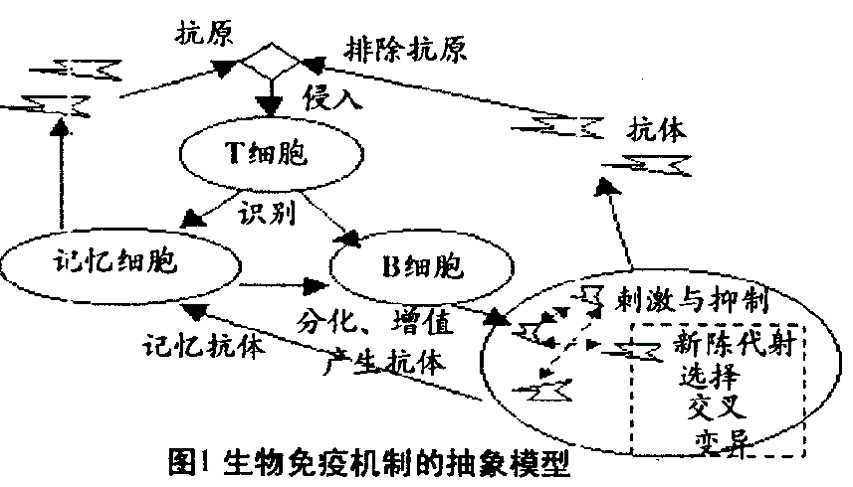
\includegraphics[scale=0.5]{img/1.png}
  \par
  
\end{frame}
\begin{frame}{Comparison of immune system and immune algorithm}
 
  
  \par
  \centering
  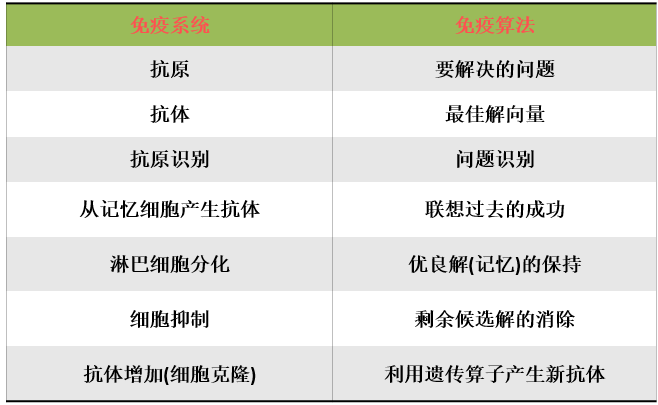
\includegraphics[scale=0.6]{img/2.PNG}
  \par
  
\end{frame}



\begin{frame}{Comparison of immune system and immune algorithm}
\par\setlength\parindent{9em}
Immune Operator:
 \par\setlength\parindent{11em}
 1.Full Immunity
 \par\setlength\parindent{11em}
 2.Target Immunity
    

     
 
\end{frame}


\begin{frame}{
Immune Operator}
\begin{block}{Full Immunity}
Full immunity refers to the type of immunity that each group of individuals in a group has an immune operation on every link after the action of genetic operators. It is mainly applied to the initial stage of individual evolution, but not in the process of evolution.
\end{block}
\begin{block}{Target Immunity}
The target immunity refers to a type of immune response at the point of action only after a genetic operation. The target immunization is generally associated with the whole process of population evolution, and it is a basic operator of the immune operation.
\end{block}

\end{frame}

\begin{frame}{Immune Algrithm}
 
 \indent 
 1.The specific analysis of the solved problems(regarded as an antigen)
 \newline
 2.This feature information is processed to transform it into a solution to the problem(The set of solutions obtained according to the scheme is called the antibody based on the vaccine above)
 \newline
 3.Transform this scheme into an immune operator in an appropriate form
 
\end{frame}

\begin{frame}{Immune algorithm based on genetic algorithm}
 
  
  \par
  \centering
  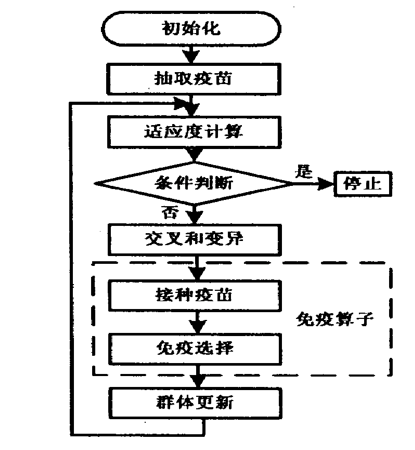
\includegraphics[scale=0.6]{img/5.PNG}
  \par
  
\end{frame}

\begin{frame}{Immune Operator}
 
 \indent 
 1.Vaccination:According to the prior knowledge, some genes in X are modified to make the individual have higher fitness for greater probability. 
 
 \newline
 
2.Immune selection:
\par\setlength\parindent{6em}
(1)Immunoassay:The detection of individuals vaccinated is not as good as the parent, indicating that the phenomenon of severe degeneration has occurred during the process of crossover and mutation, and this individual will be replaced by the corresponding individuals in the parent.
\par\setlength\parindent{6em}
(2)Annealing selection:
In the current progeny group E_k=(x_1,...,x_{n_0}), 

the individual Xi is selected by the probability $P(x_i)$ to enter the new parent group:
\par\setlength\parindent{6em}
P(x_i)=e^{f(x_i)/T_k}\sum_{i=1}^{n_0}e^{f(xi)/T_k}
\par\setlength\parindent{6em}
$f(x_i)$ is the adaptive degree of individual,
\par\setlength\parindent{6em}
$T_k$is a temperature control sequence approaching 0
 \newline
\end{frame}
\begin{frame}{Immune Operator}
 
 \indent 
$a_{H,k}^i$ is the antibody obtained after vaccinating the k generation the i individual $a_k^i$. $P_I$ is the probability of vaccinating individuals, and $P_V$ is the probability of updating the vaccine. $V(a_k^i,h_j)$ is an inoculation operation modifing the gene on an individual$a_k^i$ according to the pattern $h_j$,  and N and m are the size of the population and the vaccine, respectively.
 
 \newline
 

\par\setlength\parindent{6em}

\end{frame}

\begin{frame}{The execution algorithm of immune operator}
 
  \par\setlength\parindent{6em}
Begin:
\par\setlength\parindent{6em}
  Extraction of vaccine:
  \par\setlength\parindent{8em}
  Analyze the problem to be asked and collect the characteristic information
  \par\setlength\parindent{8em}
  Estimation of patterns on specific gene sites based on characteristic information:H={h_j|j=1,2,...,m}
   \par\setlength\parindent{6em}
   k=0andj=0;
   \par\setlength\parindent{6em}
   while(Conditions=true)
   \par\setlength\parindent{7em}
    if{P_v}=true,then j=j+1;
    \par\setlength\parindent{7em}
    i=0;
    \par\setlength\parindent{7em}
    for(i<=n)
    \par\setlength\parindent{8em}
    Vaccination:a_{H,k}^j=V_{p_I}{(a_k^i,h_j)};
    \par\setlength\parindent{8em}
    Immunoassay:if a_{H,k}^i<a_{k-1}^i,then a_k^j=a_{k-1}^i;
    else a_k^i=a_{H,k}^i;
    \par\setlength\parindent{8em}
    i=i+1;
    \par\setlength\parindent{7em}
    Annealing selection:A_{k+1}=S(A_k);
    \par\setlength\parindent{7em}
    k=k+1;
    
    End
  
  

  
\end{frame}



